\chapter{离散傅里叶变换}

本章介绍离散傅里叶变换。
广义上,离散傅里叶变换分为“离散时间傅里叶变换(Discrete-Time Fourier Transform,DTFT)”和“离散的傅里叶变换(Discrete Fourier Transform,DFT)”。
前者是对离散时域信号的变换,得到的结果依然是连续频域,后者是对频域的离散。
由于数字处理的引入,DFT是离散傅里叶学习的最终目的。

本章要点:
\begin{itemize}
    \item 离散信号的傅里叶变换,DTFT。
    \item 离散傅里叶变换,DFT。
\end{itemize}

\begin{tcolorbox}
学习DTFT和DFT,特别要注意量纲和自变量的定义域。
\end{tcolorbox}

\newpage
\section{离散信号的傅里叶变换}

本节讨论离散信号的傅里叶变换(Discrete-Time Fourier Transform,DTFT)。
相应地,连续信号的傅里叶变换称为Continuous-Time Fourier Transform,CTFT。
本节是向离散傅里叶变换(Discrete Fourier Transform,DFT)的过渡。

本节要点:
\begin{itemize}
    \item 掌握DTFT;
    \item 熟悉CTFT和DTFT的关系;
    \item 理解采样周期对DTFT的影响。
\end{itemize}

%============================================================
\subsection{DTFT的概念}

\begin{definition}[离散信号的傅里叶变换]
我们已知连续信号$x\left( t \right) $的傅里叶变换
\begin{align*}
&X\left( \omega \right) =\int_{-\infty}^{+\infty}{x\left( t \right) e^{-i\omega t}dt} \\
&x\left( t \right) =\frac{1}{2\pi}\int_{-\infty}^{+\infty}{X\left( \omega \right) e^{i\omega t}d\omega}
\end{align*}
同样我们可以定义,若离散信号$x\left[ n \right] $满足:
\begin{itemize}
    \item 任一有限区域上满足狄利克雷收敛条件,
    \item 整个实数域绝对可积,即$\sum_{n=-\infty}^{+\infty}{\left| x\left[ n \right] \right|}$收敛,
\end{itemize}
则有:
\[
x\left[ n \right] =\frac{1}{2\pi}\int_0^{2\pi}{\left[ \sum_{n=-\infty}^{+\infty}{x\left[ n \right] e^{-i\varOmega n}} \right] e^{i\varOmega n}d\varOmega}
\]
同时称$\sum_{n=-\infty}^{+\infty}{x\left[ n \right] e^{-i\varOmega n}}$为{\bf 离散信号$x\left[ n \right] $的傅里叶变换}(Discrete-Time Fourier Transform,DTFT),记为$X\left( \varOmega \right) $,即:
\[
X\left( \varOmega \right) =\sum_{n=-\infty}^{+\infty}{x\left[ n \right] e^{-i\varOmega n}}
\]
相应地称
\[
x\left[ n \right] =\frac{1}{2\pi}\int_0^{2\pi}{X\left( \varOmega \right) e^{i\varOmega n}d\varOmega}
\]
为{\bf 离散信号的傅里叶逆变换}。离散信号的傅里叶变换形式通常记为:
\[
x\left[ n \right] \overset{\mathscr{F}}{\leftrightarrow}X\left( \varOmega \right)
\]
\end{definition}

\begin{tcolorbox}
注意,为区别连续信号,离散信号的傅里叶变换的自变量通常用大写$\varOmega $表示。
其次,$X\left( \varOmega \right) $依然是连续函数。
\end{tcolorbox}

%============================================================
\subsection{DTFT的量纲}

从定义看,信号的离散化使得$n$的量纲是时间,且有$\Delta n=n-\left( n-1 \right) =1$,于是:
\[
X\left( \varOmega \right) =\sum_{n=-\infty}^{+\infty}{\left\{ x\left[ n \right] e^{-i\varOmega n}\cdot \Delta n \right\}}
\]
易得$X\left( \varOmega \right) $的量纲依然是信号的量纲除以频率的量纲$\mathrm{D}_x\cdot \mathrm{Hz}^{-1}$,和CTFT一样。
这点从逆变换形式更好理解。

$\varOmega $的量纲和$\omega $一致,表示角频。
\begin{align*}
&\because \begin{cases}
	\omega \cdot t=s\\
	\varOmega \cdot n=\varOmega \cdot \frac{t}{T_{sample}}=s\\
\end{cases} \\
&\therefore \varOmega =\omega \cdot T_{sample}=\frac{\omega}{f_{sample}}
\end{align*}
其中$s$表示弧长。
可以认为$\varOmega $和$\omega $差了一个采样频率,相当于通过$T_{sample}$做了一个尺度变换。

%============================================================
\subsection{DTFT的极坐标形式}

DTFT可以变成极坐标形式:
\begin{align*}
X\left( \varOmega \right) &=\sum_{n=-\infty}^{+\infty}{x\left[ n \right] e^{-i\varOmega n}} \\
&=\sum_{n=-\infty}^{+\infty}{x\left[ n \right] \cos \left( n\varOmega \right)}+i\sum_{n=-\infty}^{+\infty}{-x\left[ n \right] \sin \left( n\varOmega \right)} \\
&=R\left( \varOmega \right) +iI\left( \varOmega \right)
\end{align*}
于是:
\begin{align*}
&\begin{cases}
	\left| X\left( \varOmega \right) \right|=\sqrt{R^2\left( \varOmega \right) +I^2\left( \varOmega \right)}\\
	\angle X\left( \varOmega \right) =\mathrm{arc}\tan \frac{I\left( \varOmega \right)}{R\left( \varOmega \right)}\\
\end{cases} \\
&X\left( \varOmega \right) =\left| X\left( \varOmega \right) \right|\cdot e^{i\angle X\left( \varOmega \right)}
\end{align*}
同样,DTFT的幅频是偶函数,相频是奇函数,且本身有$X\left( -\varOmega \right) =\bar{X}\left( \varOmega \right) $。

%============================================================
\subsection{广义DTFT}

对于有些函数,如$x\left[ n \right] =1$等,由于不满足绝对可积条件,没有严格意义上的DTFT,但可以通过单位冲激定义广义DTFT。

假设某信号DTFT之后有$2\pi \delta \left( \varOmega \right) $,则原信号:
\begin{align*}
&\because \frac{1}{2\pi}\int_{-\pi}^{+\pi}{2\pi \delta \left( \varOmega \right) e^{i\varOmega n}d\varOmega}=\int_{-\pi}^{+\pi}{\delta \left( \varOmega \right) e^{i\varOmega n}d\varOmega}=1 \\
&\therefore 1\overset{\mathscr{F}}{\rightarrow}2\pi \delta \left( \varOmega \right)
\end{align*}
以上只是一个例子,通过$\delta \left[ n \right] $的DTFT和DTFT的性质,我们可以求得很多函数的广义DTFT。

%============================================================
\subsection{DTFT的性质}

{\bf 奇偶性}

通过DTFT的直角坐标形式易得,如果$x\left[ n \right] $是偶函数,则其DTFT是实函数,如果$x\left[ n \right] $是奇函数,则其DTFT是纯虚函数,此外,一般DTFT是$\varOmega $的复变函数。
\begin{align*}
&x\left[ n \right] \text{ is even} \quad \Rightarrow \quad X\left( \varOmega \right) =x\left[ 0 \right] +2\sum_{n=1}^{+\infty}{x\left[ n \right] \cos \left( n\varOmega \right)} \\
&x\left[ n \right] \text{ is even} \quad \Rightarrow \quad X\left( \varOmega \right) =-2i\sum_{n=1}^{+\infty}{x\left[ n \right] \sin \left( n\varOmega \right)}
\end{align*}

{\bf 周期性}

对于任何离散信号,其DTFT都是周期函数,且$T=2\pi $。
简单证明:
\begin{align*}
X\left( \varOmega +2\pi \right) &=\sum_{n=-\infty}^{+\infty}{x\left[ n \right] e^{-i\left( \varOmega +2\pi \right) n}}=\sum_{n=-\infty}^{+\infty}{x\left[ n \right] e^{-i\varOmega n}e^{-i2\pi n}} \\
&=\sum_{n=-\infty}^{+\infty}{x\left[ n \right] e^{-i\varOmega n}}
\end{align*}
可见,DTFT的周期性源于信号的离散性。
由于$X\left( \varOmega \right) $的周期性,逆变换的积分范围可以是$\left[ 0,2\pi \right] $,也可以是$\left[ -\pi ,\pi \right] $。
加之DTFT的幅频是偶函数、相频是奇函数,所以DTFT的好处是对于信号的频域分析,只需要考察$\left[ 0,\pi \right] $即可。

{\bf 采样的频域特性}

\[
\begin{cases}
	x\left[ n \right] \leftrightarrow X\left( \varOmega \right)\\
	\gamma \left( t \right) \leftrightarrow X\left( \omega \right) p_{2\pi}\left( \omega \right)\\
\end{cases} \quad \Rightarrow \quad x\left[ n \right] =\left. \gamma \left( t \right) \right|_{t=n}=\gamma \left[ n \right]
\]

这说明所谓的采样,在频域看来就是通过一个带宽$B=\pi $的低通。
或者说,采样后信号的频域从原来的整个实数限制到$\left[ -\pi ,\pi \right] $。
简单证明:
\begin{align*}
&\because \gamma \left( t \right) =\frac{1}{2\pi}\int_{-\infty}^{+\infty}{X\left( \omega \right) p_{2\pi}\left( \omega \right) e^{i\omega t}d\omega}=\frac{1}{2\pi}\int_{-\pi}^{+\pi}{X\left( \omega \right) e^{i\omega t}d\omega} \\
&\therefore \gamma \left( n \right) =\frac{1}{2\pi}\int_{-\pi}^{+\pi}{X\left( \omega \right) e^{i\omega n}d\omega}=\frac{1}{2\pi}\int_{-\pi}^{+\pi}{X\left( \varOmega \right) e^{i\varOmega n}d\varOmega}=x\left[ n \right]
\end{align*}
上述证明过程中,$t$到$n$只是一个简单的变量替换,所以,这里的“采样”固定了周期$T=1$。
如果要获得不一样的采样周期,可以先在时域做尺度变换。

{\bf 线性性}

\[
ax\left[ n \right] +by\left[ n \right] \leftrightarrow aX\left( \varOmega \right) +bY\left( \varOmega \right)
\]

{\bf 时移性、频移性}

\begin{align*}
&x\left[ n-n_1 \right] \leftrightarrow X\left( \varOmega \right) \cdot e^{-i\varOmega n_1} \\
&e^{-i\varOmega _1n}\cdot x\left[ n \right] \leftrightarrow X\left( \varOmega -\varOmega _1 \right)
\end{align*}

{\bf 反转性}

\[
x\left[ -n \right] \leftrightarrow X\left( -\varOmega \right) =\bar{X}\left( \varOmega \right)
\]

注意,DTFT没有CTFT中的“时展性”。
或者说,DTFT的“时展性”体现在对连续信号的采样周期上。
采样周期确实对DTFT结果有影响。

{\bf 三角律}

\begin{align*}
&x\left[ n \right] \cos \varOmega _1t\leftrightarrow \frac{1}{2}\left[ X\left( \varOmega +\varOmega _1 \right) +X\left( \varOmega -\varOmega _1 \right) \right] \\
&x\left[ n \right] \sin \varOmega _1t\leftrightarrow \frac{i}{2}\left[ X\left( \varOmega +\varOmega _1 \right) -X\left( \varOmega -\varOmega _1 \right) \right]
\end{align*}

{\bf 时域和}

\[
\sum_{k=1}^n{x\left[ k \right]}\leftrightarrow \frac{1}{1-e^{-i\varOmega}}X\left( \varOmega \right) +\sum_{k=-\infty}^{+\infty}{\pi X\left( 2\pi k \right) \delta \left( \pi -2\pi k \right)}
\]

{\bf 频域的微分}

\[
\left( \frac{n}{i} \right) ^m\cdot x\left[ n \right] \leftrightarrow \frac{d^mX\left( \varOmega \right)}{d\varOmega ^m}
\]

{\bf 卷积性}

\begin{align*}
&x\left[ n \right] \ast y\left[ n \right] \leftrightarrow X\left( \varOmega \right) \cdot Y\left( \varOmega \right) \\
&x\left[ n \right] \cdot y\left[ n \right] \leftrightarrow \frac{1}{2\pi}\int_{-\pi}^{+\pi}{X\left( \varOmega -\lambda \right) Y\left( \lambda \right) d\lambda}
\end{align*}

{\bf Parseval定理}

\begin{align*}
&\sum_{n=-\infty}^{+\infty}{x\left[ n \right] y\left[ n \right]}=\frac{1}{2\pi}\int_{-\pi}^{+\pi}{\bar{X}\left( \varOmega \right) Y\left( \varOmega \right) d\varOmega} \\
&\sum_{n=-\infty}^{+\infty}{x^2\left[ n \right]}=\frac{1}{2\pi}\int_{-\pi}^{+\pi}{\left| X\left( \varOmega \right) \right|^2d\varOmega}
\end{align*}

\begin{tcolorbox}
注意,DTFT没有CTFT中的“Duality”。
\end{tcolorbox}

%============================================================
\subsection{CTFT和DTFT对比}

\begin{table}[h]
\centering
% \caption{表头}
\begin{tabular}{ccc}
    \toprule
    & CTFT & DTFT\\
    \midrule
    变换 & $X\left( \omega \right) =\int_{-\infty}^{+\infty}{x\left( t \right) e^{-i\omega t}dt}$ & $X\left( \varOmega \right) =\sum_{n=-\infty}^{+\infty}{x\left[ n \right] e^{-i\varOmega n}}$\\
    逆变换 & $x\left( t \right) =\frac{1}{2\pi}\int_{-\infty}^{+\infty}{X\left( \omega \right) e^{i\omega t}d\omega}$ & $x\left[ n \right] =\frac{1}{2\pi}\int_0^{2\pi}{X\left( \varOmega \right) e^{i\varOmega n}d\varOmega}$\\
    时域变量 & 连续时间$t$ & 离散时间$n$\\
    频域变量 & 连续频率$\omega $ & 连续频率$\varOmega \in \left[ -\pi ,\pi \right] $\\
    周期 & 无 & $T=2\pi $\\
    \bottomrule
\end{tabular}
\end{table}

%============================================================
\subsection{例}

\begin{example}
设两个信号$x\left( t \right) =0.5^tu\left( t \right) ,x\left[ n \right] =0.5^nu\left[ n \right] $,分析两者的傅里叶变换。
\end{example}

$x\left( t \right) =0.5^tu\left( t \right) $的CTFT:
\begin{align*}
X\left( \omega \right) &=\int_{-\infty}^{+\infty}{0.5^tu\left( t \right) e^{-i\omega t}dt}=\int_0^{+\infty}{\left( 0.5e^{-i\omega} \right) ^tdt} \\
&=\left. \frac{\left( 0.5e^{-i\omega} \right) ^t}{\ln \left( 0.5e^{-i\omega} \right)} \right|_{0}^{+\infty}=-\frac{1}{\ln \left( 0.5e^{-i\omega} \right)}=-\frac{1}{\ln 0.5-i\omega}
\end{align*}

$x\left[ n \right] =0.5^nu\left[ n \right] $的DTFT,为公比$\left| 0.5e^{-i\varOmega} \right|<1$的无穷等比数列的和:
\[
X\left( \varOmega \right) =\sum_{n=-\infty}^{+\infty}{x\left[ n \right] e^{-i\varOmega n}}=\sum_{n=-\infty}^{+\infty}{0.5^ne^{-i\varOmega n}}=\frac{1}{1-0.5e^{-i\varOmega}}
\]

\begin{python}
t   = np.arange(0, 5, 0.01)
x_t = 0.5**t
w   = np.arange(-3*np.pi, 3*np.pi, 0.01)
X_w = -1 / (np.log(0.5) - w*1.0j)
n   = np.arange(0,26)
x_n = 0.5**(0.2*n)
W   = np.arange(-3*np.pi, 3*np.pi, 0.01)
X_W = 1 / (1 - 0.5*np.exp(-1.0j*W))

axs[0][0].plot(t, x_t)
plot_mag_phs(w, np.abs(X_w), np.angle(X_w, deg=True), ...)
axs[0][1].stem(n, x_n)
plot_mag_phs(w, np.abs(X_W), np.angle(X_W, deg=True), ...)
\end{python}

\begin{figure}[h]
\centering
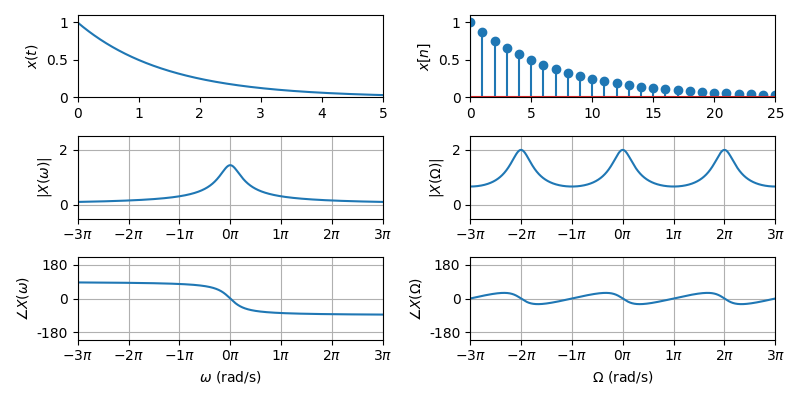
\includegraphics[height=5cm]{6.1.7-1.png}
\end{figure}

~

\begin{example}
设两个信号$x\left( t \right) =\left( -0.5 \right) ^tu\left( t \right) ,x\left[ n \right] =\left( -0.5 \right) ^nu\left[ n \right] $,(基本同上例,只是系数变成了-0.5,增强了信号波动频率),分析两者的傅里叶变换。
\end{example}

两个信号的傅里叶变换:
\begin{align*}
&\left( -0.5 \right) ^tu\left( t \right) \leftrightarrow -\frac{1}{\ln \left( -0.5 \right) -i\omega} \\
&\left( -0.5 \right) ^nu\left[ n \right] \leftrightarrow \frac{1}{1+0.5e^{-i\varOmega}}
\end{align*}

\begin{python}
t   = np.arange(0, 5, 0.01, dtype=np.complex64)
x_t = (-0.5)**t
w   = np.arange(-3*np.pi, 3*np.pi, 0.01)
X_w = -1 / (np.log(-0.5+0.0j) - 1.0j*w)
n   = np.arange(0,26, dtype=np.complex64)
x_n = (-0.5)**(0.2*n)
W   = np.arange(-3*np.pi, 3*np.pi, 0.01)
X_W = 1 / (1 + 0.5*np.exp(-1.0j*W))

axs[0][0].plot(t.real, x_t.real)
plot_mag_phs(w, np.abs(X_w), np.angle(X_w, deg=True), ...)
axs[0][1].stem(n.real, x_n.real)
plot_mag_phs(w, np.abs(X_W), np.angle(X_W, deg=True), ...)
\end{python}

\begin{figure}[h]
\centering
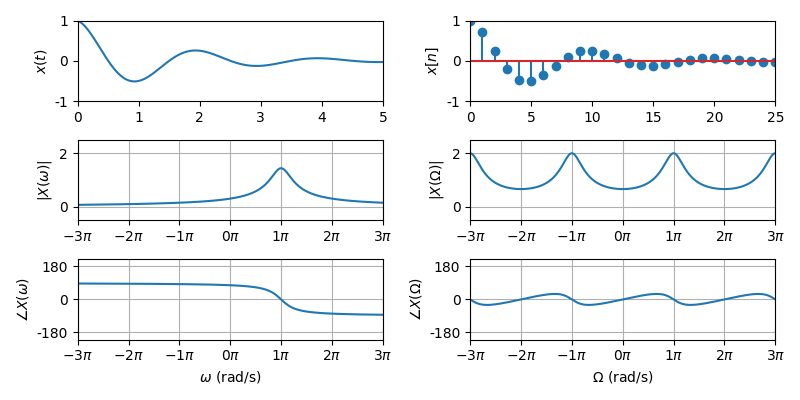
\includegraphics[height=5cm]{6.1.7-2.png}
\end{figure}

\begin{itemize}
    \item DTFT依然呈现周期性;
    \item 对比两个FT,0.5的FT集中在低频,-0.5的FT集中在高频。
\end{itemize}

%============================================================
\subsection{采样周期对DTFT的影响}

从量纲分析可得,DTFT和CTFT两者的意义相同,区别只在于变量。
由于对时域信号做了采样,所以暂时可以认为$\varOmega $对于$\omega $做了尺度变换,$\varOmega =\omega \cdot T_{sample}$。
而且通常$T_{sample}<1$,相当于信号变慢。
所以随着采样频率的提高,DTFT结果会向低频段集中。

实际上,DTFT的频率范围只是$\left[ -\pi ,\pi \right] $,其他部分都是周期性的复现。
由于对称性,实际分析的只是$\left[ 0,\pi \right] $,称为“窗口”。
DTFT在频率轴上开了一个窗口,将CTFT的频率“映射”到$\left[ 0,\pi \right] $,通过采样频率将CTFT的$0\text{~}\pi \cdot f_{sample}$部分映射到窗口中。
所以采样频率越高,我们在DTFT上看到的频率越宽广。

用前面的例子说明。
假设时域信号$x\left( t \right) =\left( -0.5 \right) ^t\cdot u\left( t \right) $,分析采样周期$T$对DTFT的影响。

令$t=nT$进行离散化,得到DTFT结果:
\begin{align*}
x\left[ n \right] &=\left( -0.5 \right) ^{nT}=\left[ \left( -0.5 \right) ^T \right] ^n \\
X\left( \varOmega \right) &=\sum_{n=-\infty}^{+\infty}{x\left[ n \right] e^{-i\varOmega n}}=\sum_{n=-\infty}^{+\infty}{\left[ \left( -0.5 \right) ^T \right] ^ne^{-i\varOmega n}} \\
&=\frac{1}{1-\left( -0.5 \right) ^Te^{-i\varOmega}}
\end{align*}
\begin{figure}[h]
\centering
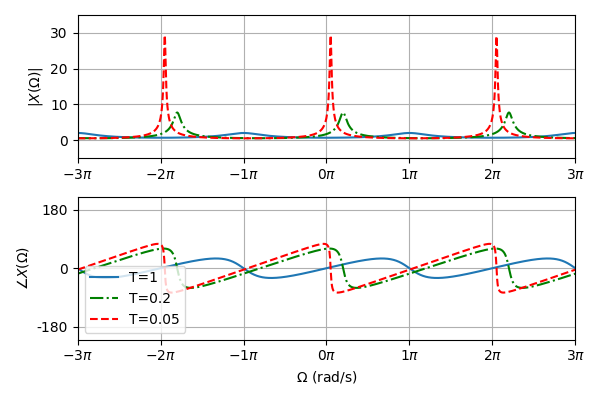
\includegraphics[height=5cm]{6.1.8-1.png}
\end{figure}

\begin{python}
W = np.arange(-3*np.pi, 3*np.pi, 0.01)
T = 1;    X_1 = 1 / (1 - (-0.5)**T * np.exp(-1.0j*W))
T = 0.2;  X_2 = 1 / (1 - (-0.5)**T * np.exp(-1.0j*W))
T = 0.05; X_3 = 1 / (1 - (-0.5)**T * np.exp(-1.0j*W))

plot_mag_phs(W, np.abs(X_1), np.angle(X_1, deg=True),
             mag_line_fmt='-', phs_line_fmt='-',
             mag_line_label='T=1', phs_line_label='T=1')
plot_mag_phs(W, np.abs(X_2), np.angle(X_2, deg=True),
             mag_line_fmt='g-.', phs_line_fmt='g-.',
             mag_line_label='T=0.2', phs_line_label='T=0.2')
plot_mag_phs(W, np.abs(X_3), np.angle(X_3, deg=True),
             mag_line_fmt='r--', phs_line_fmt='r--',
             mag_line_label='T=0.05', phs_line_label='T=0.05')
\end{python}

注意:
\begin{itemize}
    \item $T=1$时,可以认为就是原信号,即$X\left( \varOmega \right) =X\left( \omega \right) $。
    \item 随着采样频率的提高,DTFT窗口看到的频率越宽,使得“峰越往低频方向偏移”,或者认为在同样的 的“步频”下,采样频率越高信号“走得越慢”。
\end{itemize}






\newpage
\section{基于DTFT的系统频域分析}

本节在频域角度,讨论离散系统的响应。

本节要点:
\begin{itemize}
    \item 离散系统频率响应的概念;
    \item 了解采样频率对输出的影响。
\end{itemize}

%============================================================
\subsection{离散系统的频域响应定理}

\begin{theorem}[离散系统的频域响应定理]
如果一个零状态LTI系统满足绝对稳定的条件,即$\sum_{n=-\infty}^{+\infty}{\left| h\left[ n \right] \right|}<\infty $,则系统对于任意非周期信号$x\left[ n \right] $在时域的输出可以表示为卷积:
\[
y\left[ n \right] =x\left[ n \right] \ast h\left[ n \right]
\]
在频域的输出可以表示为DTFT的乘积:
\[
Y\left( \varOmega \right) =X\left( \varOmega \right) \cdot H\left( \varOmega \right)
\]
\begin{itemize}
    \item $x\left[ n \right] ,y\left[ n \right] $:输入输出信号的时域表达式;
    \item $h\left[ n \right] $:系统的冲激响应;
    \item $X\left( \varOmega \right) ,Y\left( \varOmega \right) $:输入输出信号的DTFT;
    \item $H\left( \varOmega \right) $:{\bf 离散系统的频率响应函数}(frequency response function),或称{\bf 系统函数}(system function),即$h\left[ n \right] $的傅里叶变换。
\end{itemize}
\end{theorem}

一个满足绝对稳定条件的LTI系统对任何输入的信号,系统会单独作用其各个频率分量的幅度和相位:
\begin{align*}
&\left| Y\left( \varOmega \right) \right|=\left| X\left( \varOmega \right) \right|\cdot \left| H\left( \varOmega \right) \right| \\
&\angle Y\left( \varOmega \right) =\angle X\left( \varOmega \right) +\angle H\left( \varOmega \right)
\end{align*}

%============================================================
\subsection{理想低通和采样频率对信号的影响}

数字系统对时域信号通常的做法是先采样进行离散化,再通过一个数字滤波器。
这里考察数字滤波器(即系统本身)和采样过程对信号通过性的影响。

首先考察滤波器对信号的输出结果。
由于DTFT的周期性,离散系统的频率响应函数是一个$T=2\pi $的周期函数。
假设一LTI离散系统(理想低通)有如下频率响应函数:
\begin{figure}[ht]
\centering
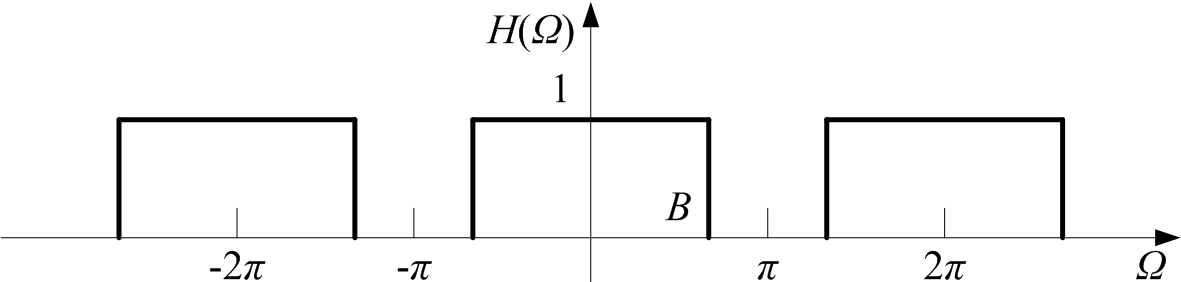
\includegraphics[height=2.5cm]{6.2.2-1.png}
\end{figure}
\[
H\left( \varOmega \right) =\sum_{n=-\infty}^{+\infty}{p_{2B}\left( \varOmega +2\pi n \right)}
\]

对比CTFT的系统频域分析,这里要注意几点:
\begin{itemize}
    \item 由于DTFT的周期性,一般考察区间$\left[ -\pi ,\pi \right] $,往0方向的是低频,往$\pm \pi $方向的是高频。
    \item 由于的频谱的对称性,考察区间可缩小为$\left[ 0,\pi \right] $。
\end{itemize}

\begin{tcolorbox}
这样的理想低通是不存在的,因为其冲激响应$h\left[ n \right] =\frac{B}{\pi}\sin\mathrm{c}\left( \frac{B}{\pi}n \right) $不符合因果性。
\end{tcolorbox}

对于简单的正弦信号$x\left[ n \right] =A\cos \left( \varOmega _0n \right) $,其DTFT有
\[
X\left( \varOmega \right) =\sum_{m=-\infty}^{\infty}{A\pi \left[ \delta \left( \varOmega +\varOmega \,\,_0+2\pi m \right) +\delta \left( \varOmega -\varOmega \,\,_0+2\pi m \right) \right]}
\]
只要$\varOmega _0\leqslant B$,信号就能通过该系统,如下图。
\begin{figure}[h]
\centering
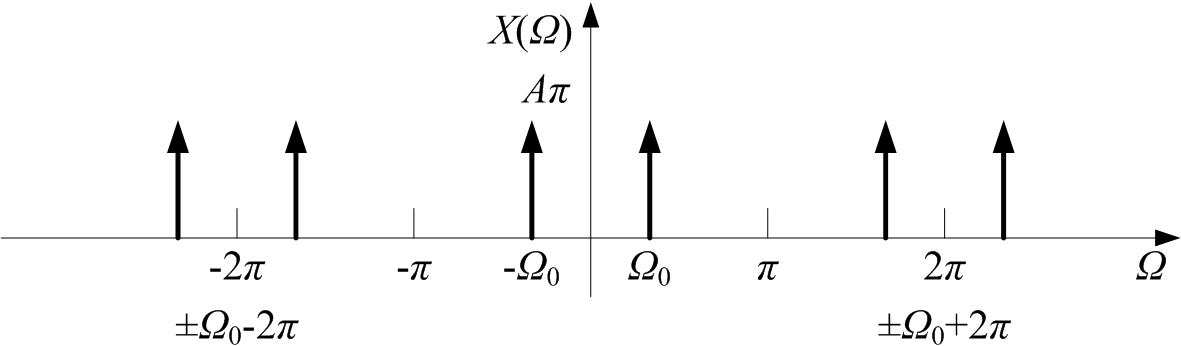
\includegraphics[height=3cm]{6.2.2-2.png}
\end{figure}

再考察采样对输出的影响。
假设连续时域信号$x\left( t \right) =A\cos \left( \omega _0t \right) $,对其采样
\begin{align*}
&x\left[ n \right] =\left. x\left( t \right) \right|_{t=nT}=A\cos \left( \omega _0nT \right) \overset{\varOmega _0=\omega _0T}{=}A\cos \left( \varOmega _0n \right) \\
&n=0,\pm 1,\pm 2,\cdots
\end{align*}
要使$\varOmega _0\leqslant B$,即$\omega _0T\leqslant B$,也即$T\leqslant B/\omega _0$。

\begin{tcolorbox}
采样频率越高,DTFT映射到的实际频率范围越宽。
\end{tcolorbox}

%============================================================
\subsection{均值滤波器}

考虑最简单的平均化,系统的输入输出差分方程为:
\[
y\left[ n \right] =\frac{1}{N}\sum_{k=0}^{N-1}{x\left[ n-k \right]}
\]
一般认为当$N\geqslant 3$时有较为锋利的截止,这样的系统称为{\bf 均值滤波器}(mean filter),频率响应函数:
\begin{align*}
&\because h\left[ n \right] =\frac{1}{N}\sum_{k=0}^{N-1}{\delta \left[ n-k \right]} \\
&\because \begin{cases}
	x\left[ n-n_1 \right] \leftrightarrow X\left( \varOmega \right) \cdot e^{-i\varOmega n_1}\\
	\delta \left[ n \right] \leftrightarrow 1\\
\end{cases} \\
&\therefore H\left( \varOmega \right) =\frac{1}{N}\sum_{k=0}^{N-1}{e^{-i\varOmega k}}
\end{align*}

\begin{python}
def mean_filter(N, W):
	H = 1
	for i in range(1, N):
		H = H + np.exp(-1.0j * i * W)
		pass
	H = H / N
	return H

W  = np.arange(-3*np.pi, 3*np.pi, 0.01)
N1 = 2;  H1 = mean_filter(N1, W)
N2 = 5 ; H2 = mean_filter(N2, W)
N3 = 20; H3 = mean_filter(N3, W)

plot_mag_phs(W, np.abs(H1), np.angle(H1, deg=True), ...)
plot_mag_phs(W, np.abs(H2), np.angle(H2, deg=True), ...)
plot_mag_phs(W, np.abs(H3), np.angle(H3, deg=True), ...)
\end{python}

\begin{figure}[h]
\centering
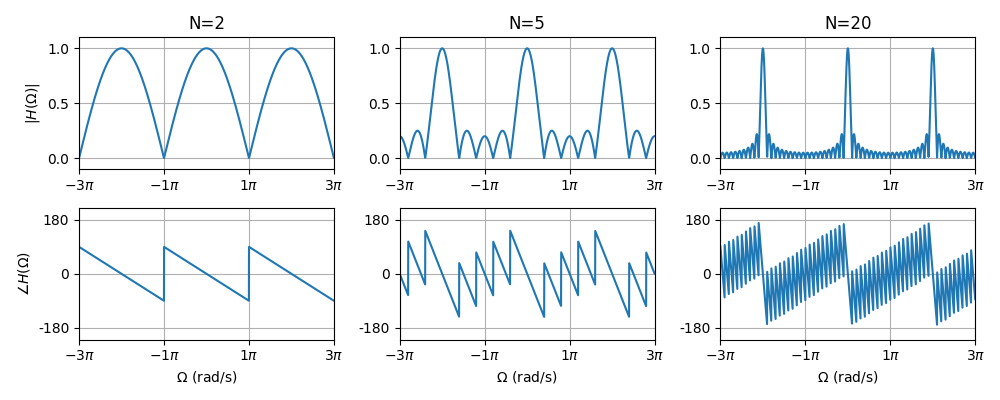
\includegraphics[height=4cm]{6.2.3-1.png}
\end{figure}

由幅频图可得系统是个低通,且阶数越高带宽越小,时域上就是抹得越平。






\newpage
\section{离散傅里叶变换}

之前的章节,从CTFT到DTFT,完成了从连续信号到离散信号的傅里叶分析。
\[
\begin{cases}
	X\left( \omega \right) =\int_{-\infty}^{+\infty}{x\left( t \right) e^{-i\omega t}dt}\\
	x\left( t \right) =\frac{1}{2\pi}\int_{-\infty}^{+\infty}{X\left( \omega \right) e^{i\omega t}d\omega}\\
\end{cases}\,\,  \Rightarrow \,\,  \begin{cases}
	X\left( \varOmega \right) =\sum_{n=-\infty}^{+\infty}{x\left[ n \right] e^{-i\varOmega n}}\\
	x\left[ n \right] =\frac{1}{2\pi}\int_{-\infty}^{+\infty}{X\left( \varOmega \right) e^{i\varOmega t}d\varOmega}\\
\end{cases}
\]
DTFT从非周期性的连续谱变成周期性的连续谱($0\text{~}2\pi $的稠密的连续谱)。
本节介绍对DTFT的离散化,获得一个离散的傅里叶变换结果。

本节要点:
\begin{itemize}
    \item 掌握DFT;
    \item 熟悉CTFT、DTFT和DFT三者关系;
    \item 掌握DFT的Python实现;
    \item 充分理解采样频率和采样数量对DFT的影响。
\end{itemize}

%============================================================
\subsection{DFT的概念}

\begin{definition}[离散傅里叶变换]
假设离散信号$x\left[ n \right] $只在$n\in \left[ 0,N \right) $上有定义(即$n=0,1,2,\cdots ,N-1$,一般$N$很大,如1024),则称:
\[
X\left[ m \right] =\sum_{n=0}^{N-1}{x\left[ n \right] e^{-i\left( \frac{2\pi}{N}m \right) n}} \qquad m=0,1,2,\cdots ,N-1
\]
为{\bf 离散信号$x\left[ n \right] $的离散傅里叶变换}(Discrete Fourier Transform,DFT)。
相应地称
\[
x\left[ n \right] =\frac{1}{N}\sum_{m=0}^{N-1}{X\left[ m \right] e^{i\left( \frac{2\pi}{N}n \right) m}} \qquad n=0,1,2,\cdots ,N-1
\]
为{\bf 离散傅里叶逆变换}(inverse Discrete Fourier Transform,iDFT)。
离散信号的傅里叶变换形式通常记为:
\[
x\left[ n \right] \overset{\mathscr{F}}{\leftrightarrow}X\left[ m \right]
\]
\end{definition}

由于DFT和iDFT都是有限和,所以离散傅里叶变换和逆变换总是存在的。其次,由于DFT的求和区间是$\left[ 0,N \right) $,所以DFT不是周期函数。

%============================================================
\subsection{DFT的量纲}

由于这里$N$的带有信号总时长的属性,可以认为有时间量纲,所以$X\left[ m \right] $的量纲依然是信号量纲除以频率($\mathrm{D}_x\cdot \mathrm{Hz}^{-1}$),表示单位频率的信号的量,即信号的频率密度。
如果考虑到$n,N$的时间量纲属性,$m$无量纲。
如果考虑到$t=n\cdot T_{sample}$,则有
\begin{align*}
&\because \begin{cases}
	\omega \cdot t=s\\
	\frac{2\pi}{N}\cdot m\cdot \frac{t}{T_{sample}}=s\\
\end{cases} \\
&\therefore \omega =\frac{2\pi}{N}\cdot m\cdot \frac{1}{T_{sample}}=\frac{\omega _{sample}}{N}\cdot m
\end{align*}
其中$s$表示弧长。
$m$依然无量纲。
但其物理意义很清楚,对于采样频率$N$等分之后的序数。
可令基频$\omega _0=\frac{\omega _{sample}}{N}$,则有$\omega =m\omega _0$。
$X\left[ m \right] $代表信号在频率$\frac{\omega _{sample}}{N}\cdot m$(或$\frac{f_{sample}}{N}\cdot m$)处的分量,且$m\in \left[ 0,N \right) $。

~

若采样频率1000Hz,采样100个数据$x\left[ 0 \right] \text{~}x\left[ 99 \right] $,DFT之后得到100个频域数据$X\left[ 0 \right] \text{~}X\left[ 99 \right] $。
由于对称性,只需要考察$X\left[ 0 \right] \text{~}X\left[ 49 \right] $。
$X\left[ 0 \right] $表示信号的直流分量,$X\left[ 1 \right] $表示信号$\frac{1000\mathrm{Hz}}{100}\cdot 1=10\mathrm{Hz}$的分量,以此类推,$X\left[ 49 \right] $表示信号$\frac{1000\mathrm{Hz}}{100}\cdot 49=490\mathrm{Hz}$的分量。
特别注意,由于对称性$X\left[ 99 \right] $表示信号10Hz的分量!

从上述分析可以得到:
\begin{itemize}
    \item 采样频率越高,越能看到信号的高频,即若要分析某信号位于$f_0$的分量,则采样频率至少需要其两倍$f_{sample}=2f_0$。
    \item 采样数据决定了频谱的分辨率,若频谱要看的细致,则必须采集更多的信号值。
\end{itemize}
即,采样频率决定了DFT的呈现范围,采样量决定了DFT的细腻程度。

%============================================================
\subsection{DFT的直角坐标形式}

DFT的直角坐标形式:
\begin{align*}
&X\left[ m \right] =\sum_{n=0}^{N-1}{x\left[ n \right] e^{-i\left( \frac{2\pi}{N}n \right) m}} \\
&=\sum_{n=0}^{N-1}{x\left[ n \right] \cos \left( \frac{2\pi n}{N}m \right)}+i\sum_{n=0}^{N-1}{-x\left[ n \right] \sin \left( \frac{2\pi n}{N}m \right)} \\
&\begin{cases}
	R\left[ m \right] =\sum_{n=0}^{N-1}{x\left[ n \right] \cos \left( \frac{2\pi n}{N}m \right)}=x\left[ 0 \right] +\sum_{n=1}^{N-1}{x\left[ n \right] \cos \frac{2\pi nm}{N}}\\
	I\left[ m \right] =\sum_{n=0}^{N-1}{-x\left[ n \right] \sin \left( \frac{2\pi n}{N}m \right)}=-\sum_{n=1}^{N-1}{x\left[ n \right] \sin \frac{2\pi nm}{N}}\\
\end{cases}
\end{align*}

由于DFT的求和区间是$\left[ 0,N \right) $,而非像DTFT一样区间关于原点对称,所以信号的奇偶性并不影响DFT的复变函数形式。

%============================================================
\subsection{Python应用——DFT和iDFT函数}

这里,我们编写两个Python函数(my\_dft和my\_idft)用以求解有限离散信号的DFT和iDFT:
\begin{align*}
&X\left[ m \right] =\sum_{n=0}^{N-1}{x\left[ n \right] e^{-i\left( \frac{2\pi}{N}m \right) n}} \qquad m=0,1,2,\cdots ,N-1 \\
&x\left[ n \right] =\frac{1}{N}\sum_{m=0}^{N-1}{X\left[ m \right] e^{i\left( \frac{2\pi}{N}n \right) m}} \qquad n=0,1,2,\cdots ,N-1
\end{align*}

\begin{python}
def my_dft(x:np.ndarray) -> np.ndarray:
    X = np.zeros_like(x, dtype=np.complex64)
    N = x.size
    n = np.arange(0, x.size)
    for m in range(0, x.size):
        X[m] = np.dot(x, np.exp(0-1.0j*2*np.pi*m*n/N))
    return X

def my_idft(X:np.ndarray) -> np.ndarray:
    x = np.zeros_like(X, dtype=np.float64)
    M = X.size
    m = np.arange(0, X.size)
    for n in range(0, X.size):
        x[n] = np.dot(X, np.exp(0+1.0j*2*np.pi*m*n/M)) / M
        pass
    return x
\end{python}

%============================================================
\subsection{CTFT、DTFT和DFT三者关系}

{\bf CTFT}

\begin{align*}
&X\left( \omega \right) =\int_{-\infty}^{+\infty}{x\left( t \right) e^{-i\omega t}dt} \qquad \omega \in \mathbb{R} \\
&x\left( t \right) =\frac{1}{2\pi}\int_{-\infty}^{+\infty}{X\left( \omega \right) e^{i\omega t}d\omega} \qquad t\in \mathbb{R}
\end{align*}

{\bf DTFT}

\begin{align*}
&X\left( \varOmega \right) =\sum_{n=-\infty}^{+\infty}{x\left[ n \right] e^{-i\varOmega n}} \qquad \varOmega \in \left[ 0,2\pi \right) \\
&x\left[ n \right] =\frac{1}{2\pi}\int_0^{2\pi}{X\left( \varOmega \right) e^{i\varOmega n}d\varOmega} \qquad n\in \mathbb{Z}
\end{align*}

{\bf DFT}

\begin{align*}
&X\left[ m \right] =\sum_{n=0}^{N-1}{x\left[ n \right] e^{-i\frac{2\pi mn}{N}}} \qquad m\in \left[ 0,N \right) \\
&x\left[ n \right] =\frac{1}{N}\sum_{m=0}^{N-1}{X\left[ m \right] e^{i\frac{2\pi nm}{N}}} \qquad n\in \left[ 0,N \right)
\end{align*}

进一步对比DTFT和DFT对频率的处理,假设$x\left[ n \right] $只在$n\in \left[ 0,N \right) $上有定义,则:
\begin{align*}
&X\left( \varOmega \right) =\sum_{n=-\infty}^{+\infty}{x\left[ n \right] e^{-i\varOmega n}}=\sum_{n=0}^{N-1}{x\left[ n \right] e^{-i\varOmega n}} \\
&X\left[ m \right] =\sum_{n=0}^{N-1}{x\left[ n \right] e^{-i\left( \frac{2\pi}{N}m \right) n}}
\end{align*}
两者差别在于DFT将DTFT的连续频域变量$\varOmega $离散化为$m$,或者说对频域进行了采样,间隔为$2\pi /N$,采样$N$个点:
\[
\varOmega \,\,=\frac{2\pi}{N}m \qquad m=0,1,2,\cdots ,N-1
\]

%============================================================
\subsection{采样频率和采样数量对DFT的影响}

\begin{figure}[h]
\centering
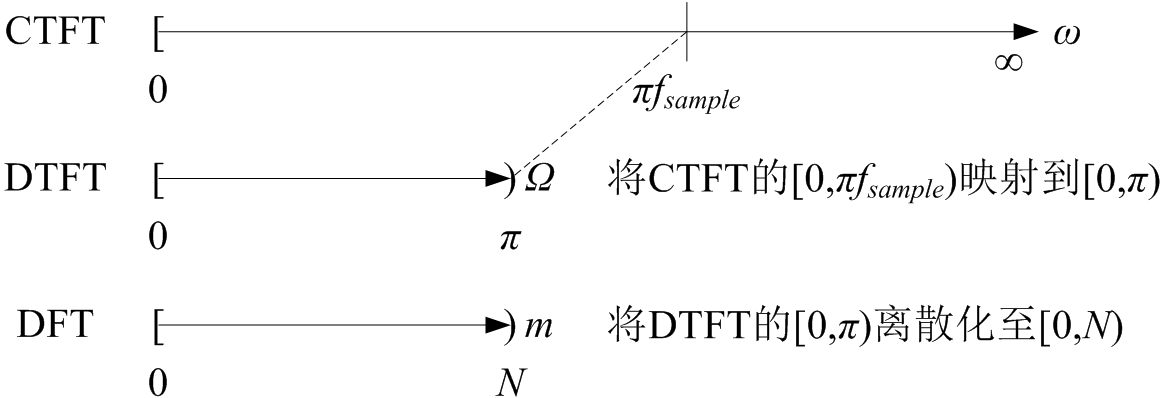
\includegraphics[height=3cm]{6.3.6-1.png}
\end{figure}

{\bf 采样频率$f_{sample}$的影响}

DTFT将CTFT的$0\text{~}\pi \cdot f_{sample}$部分映射到窗口$\left[ 0,\pi \right] $中,所以采样频率决定DTFT能看到多高频率范围,$f_{sample}$越高,越能收集信号的变化,对应地DTFT越能看到高频,越逼近CTFT。

{\bf 采样数量$N$的影响}

DFT再将DTFT的窗口离散化成$\left[ 0,N/2 \right) $,$X\left[ m \right] $的整体包络就是$X\left( \varOmega \right) $,所以信号序列的长度(即$N$)并不改变$X\left[ m \right] $的整体形状,$N$越大,表示对信号收集地越多,DFT越密集、分辨率越高、越细腻,越能精确描述包络形状,越贴近对应的$X\left( \varOmega \right) $曲线。

综合来讲,对于同样的信号,$f_{sample}$决定了你能看到多宽的频率(即频率的上限),$N$决定了你能看到多细腻的频谱,或者说DFT和CTFT的“长相一致程度”。

~

\begin{example}
假设有一个方波信号,前10秒是1,后面都是0,分析不同的采样数量和不同的采样频率对DFT的影响。
\end{example}

信号及其傅里叶变换如下图:
\begin{figure}[h]
\centering
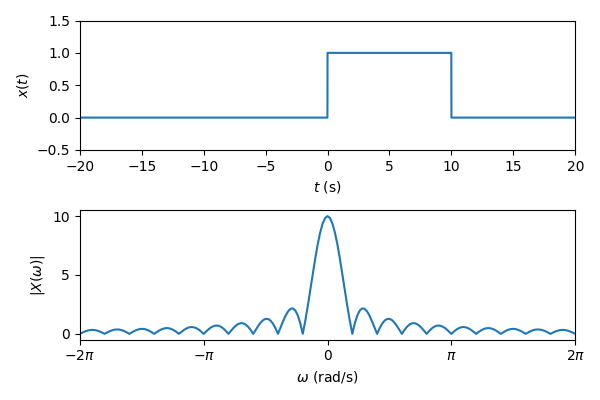
\includegraphics[height=4cm]{6.3.6-2.png}
\end{figure}

先分析不同的采样数量对DFT的影响,假设采样周期1s,即:
\[
x\left[ n \right] =1 \qquad n=0,1,2,3,4,5,6,7,8,9
\]
取三个不同的采样数量(10s,20s,110s),用Python计算DFT并作图:

\begin{python}
n_1  = np.arange(0, 10)
xn_1 = np.ones(10)
Xm_1 = my_dft(xn_1)

n_2  = np.arange(0, 20)
xn_2 = np.where(n_2<10, 1, 0)
Xm_2 = my_dft(xn_2)

n_3  = np.arange(0, 110)
xn_3 = np.where(n_3<10, 1, 0)
Xm_3 = my_dft(xn_3)

axs[0].stem(n_1, np.abs(Xm_1))
axs[1].stem(n_2, np.abs(Xm_2))
axs[2].stem(n_3, np.abs(Xm_3))
\end{python}

\begin{itemize}
    \item 如果采样数量小于等于方波,则这个序列其实可以认为是$x\left[ n \right] =1$,DFT也说明了这个问题;
    \item 采样数量越多,越能说明原连续信号,DFT的结果约贴近CTFT,结合量纲分析,就是频谱的分辨率更高。
\end{itemize}

\begin{figure}[ht]
\centering
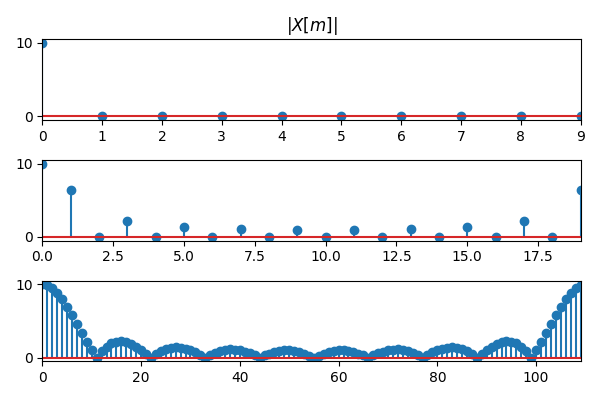
\includegraphics[height=5cm]{6.3.6-3.png}
\end{figure}

再分析采样频率对DFT的影响,分别用三种不同的采样频率(1s,0.5s,0.2s),采样数量都为50s,用Python计算DFT并作图:

\begin{python}
n_1  = np.arange(0, 50)
xn_1 = np.where(n_1<10, 1, 0)
Xm_1 = my_dft(xn_1)

n_2  = np.arange(0, 100)
xn_2 = np.where(n_2<20, 1, 0)
Xm_2 = my_dft(xn_2)

n_3  = np.arange(0, 250)
xn_3 = np.where(n_3<50, 1, 0)
Xm_3 = my_dft(xn_3)

axs[0].plot(n_1, np.abs(Xm_1))
axs[1].plot(n_2, np.abs(Xm_2))
axs[2].plot(n_3, np.abs(Xm_3))
\end{python}

\begin{figure}[h]
\centering
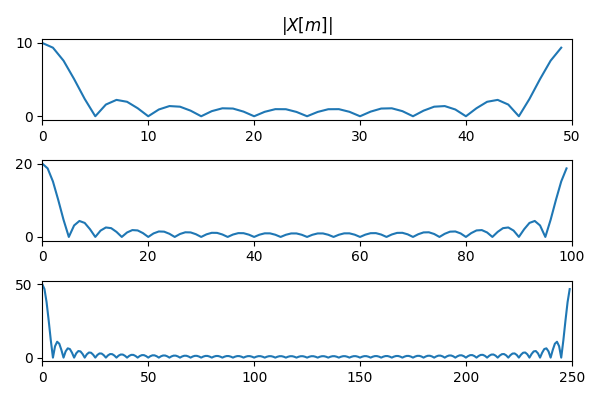
\includegraphics[height=5cm]{6.3.6-4.png}
\end{figure}

\begin{itemize}
    \item 为了看清,使用plot函数作图;
    \item 采样频率影响DFT的大致形状;
    \item 采样频率不影响lobe的“宽度”(即DFT两个相邻0值的间隔距离),影响lobe的“厚度”;
    \item 采样频率越高,频率范围越“拥挤”,即可看到的频率越多,结合量纲分析就是越能看到高频部分;
    \item 采样频率越高,DFT低频份量占比越多,这和采样周期对DTFT的影响的分析一致。
\end{itemize}

%============================================================
\subsection{填充技术对DFT的影响}

虽然采样数量越多,DFT越能体现CTFT,但真实系统对采样数量还是有要求的,采样数量不可能无限多。
这里讨论一种填充技术,书中称为“DFT of truncated signal”。

如下连续信号,以$T=0.5$采样,信号及其傅里叶变换如下:
\begin{align*}
&x\left( t \right) =0.9^t \qquad t\geqslant 0 \\
&X\left( \omega \right) =-\frac{1}{\ln 0.9-i\omega}
\end{align*}
\begin{figure}[h]
\centering
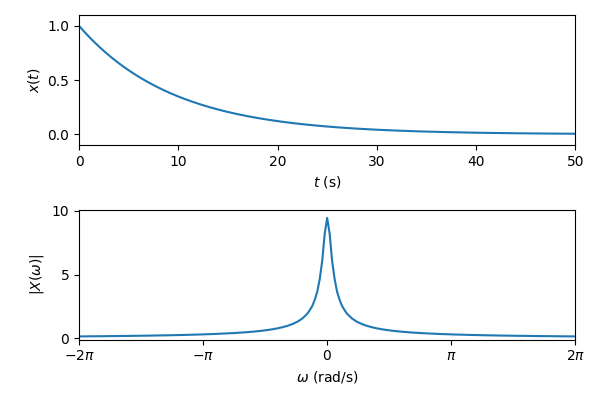
\includegraphics[height=4cm]{6.3.7-1.png}
\end{figure}
% \begin{figure}[h]
% \centering
%     \begin{minipage}{0.48\linewidth}
%     \centerline{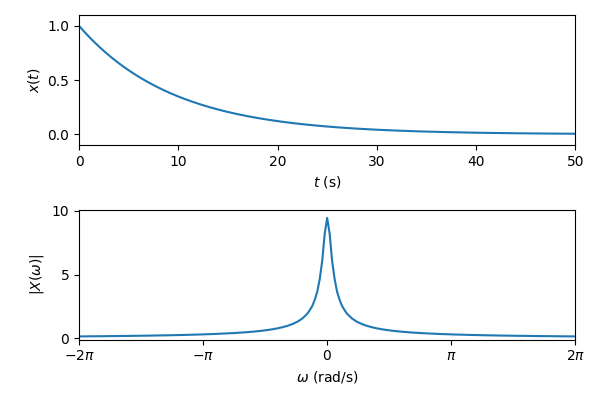
\includegraphics[height=4cm]{6.3.7-1.png}}
%     \end{minipage}
% \hfill
%     \begin{minipage}{0.48\linewidth}
%     \begin{align*}
%     &x\left( t \right) =0.9^t \qquad t\geqslant 0 \\
%     &X\left( \omega \right) =-\frac{1}{\ln 0.9-i\omega}
%     \end{align*}
%     \end{minipage}
% \end{figure}

使用Python辅助分析:
\begin{python}
n_1  = np.arange(0, 30, 0.5)
xn_1 = 0.9**n_1
Xm_1 = my_dft(xn_1)

n_2  = np.arange(0, 10, 0.5)
xn_2 = 0.9**n_2
Xm_2 = my_dft(xn_2)

n_3  = np.arange(0, 30, 0.5)
xn_3 = 0.9**n_3; xn_3[xn_2.size:] = 0
Xm_3 = my_dft(xn_3)

axs[0].plot(np.abs(Xm_1))
axs[1].plot(np.abs(Xm_2))
axs[2].plot(np.abs(Xm_3))
\end{python}

\begin{itemize}
    \item 足额采样,xn\_1采样前30s,DFT结果Xm\_1大致能体现CTFT,如下第一幅;
    \item 采样不足,xn\_2只采样前10s,DFT结果Xm\_2开始有明显失真,如下第二幅。
    \item 填充技术弥补采样不足,xn\_2只采样前10s,后20s人为填充0,相当于时域叠加了方波,DFT结果Xm\_3叠加了sinc函数,如下第三幅。
\end{itemize}

\begin{figure}[h]
\centering
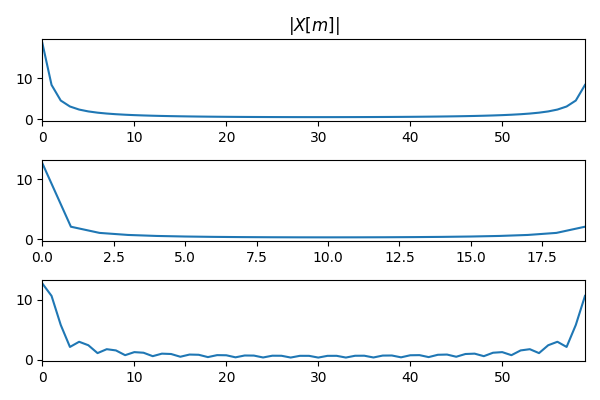
\includegraphics[height=5cm]{6.3.7-2.png}
\end{figure}

填充技术其实是一种“伪细腻化”技术,填充的值越接近实际信号,越接近真实的细腻。






\newpage
\section{离散傅里叶变换的性质}

本节介绍DFT的性质。
由于DFT的定义域受限,所以在做坐标平移时和DTFT不同。

本节要点:
\begin{itemize}
    \item 理解循环平移(时移和频移);
    \item 掌握循环卷积。
\end{itemize}

%============================================================
\subsection{循环时移和循环频移}

\begin{definition}[循环时移]
假设离散信号$x\left[ n \right] ,n\in \left[ 0,N \right) $,当有$q\in \mathbb{Z} $,$x\left[ n-q \right] $的超出定义域部分值挪到另一边,这样的时移称为{\bf 循环时移},记为$x\left[ n-q,\mathrm{mod}N \right] $,即:
\[
x\left[ n-q,\mathrm{mod}N \right] =\begin{cases}
	x\left[ N-q \right]&		n=0\\
	x\left[ N-q+1 \right]&		n=1\\
	\vdots&		\\
	x\left[ N-1 \right]&		n=q-1\\
	x\left[ 0 \right]&		n=q\\
	x\left[ 1 \right]&		n=q+1\\
	\vdots&		\\
	x\left[ N-q-1 \right]&		n=N-1\\
\end{cases}
\]
\end{definition}

离散信号的循环时移可以用圆助记,信号$x\left[ n \right] ,n\in \left[ 0,N \right) $可以认为是$N$个以逆时针方向平均分布在一单位圆上的点集,可取正下方为$x\left[ 0 \right] $。
$x\left[ n-q,\mathrm{mod}N \right] ,q>0$为将圆逆时针转$q$格。
例如$x\left[ n-3,\mathrm{mod}8 \right] $:
\begin{figure}[h]
\centering
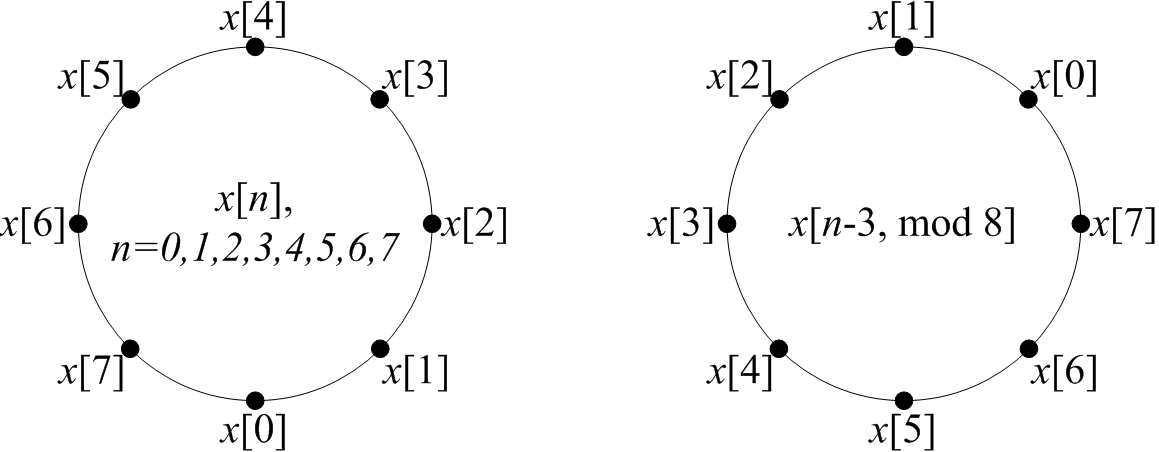
\includegraphics[height=4cm]{6.4.1-1.png}
\end{figure}

同样可以定义{\bf 循环频移}$X\left[ m-q,\mathrm{mod}N \right] $,略。

%============================================================
\subsection{循环卷积}

之前定义了离散函数的卷积:
\[
a\left[ n \right] \ast b\left[ n \right] =\sum_{i=-\infty}^{+\infty}{a\left[ i \right] b\left[ n-i \right]}
\]
由于DFT中信号只在$\left[ 0,N \right) $上有定义,所以可以仿照循环时移的定义,定义一个循环的卷积。

\begin{definition}[循环卷积]
对于两个离散函数$a\left[ n \right] ,b\left[ n \right] ,n\in \left[ 0,N \right) $,我们称和式$\sum_{i=0}^{N-1}{a\left[ i \right] b\left[ n-i,\mathrm{mod}N \right]}$为$a\left[ n \right] ,b\left[ n \right] $的{\bf 循环卷积}(circular convolution),记为$a\left[ n \right] \circledast b\left[ n \right] $,即:
\[
a\left[ n \right] \circledast b\left[ n \right] =\sum_{i=0}^{N-1}{a\left[ i \right] b\left[ n-i,\mathrm{mod}N \right]}
\]
为表区分,特别将前者称为{\bf 线性卷积}(linear convolution)。
\end{definition}

\begin{theorem}[卷积相等定理]
若有两个离散函数$a\left[ n \right] ,b\left[ n \right] ,n\in \left[ 0,N \right) $,如果将其零项扩充至$2N-2$,即:
\[
a\left[ n \right] =b\left[ n \right] =0 \qquad n\in \left[ N,2N-1 \right)
\]
则离散函数$a\left[ n \right] =b\left[ n \right] =0,n\in \left[ N,2N-1 \right) $的线性卷积和循环卷积结果一致,即:
\[
a\left[ n \right] \ast b\left[ n \right] =a\left[ n \right] \circledast b\left[ n \right]
\]
\end{theorem}

所以通常来讲,DFT和DTFT结果是不一致的,除非对信号进行零扩充。

%============================================================
\subsection{DFT的性质}

{\bf 线性性}
\[
ax\left[ n \right] +by\left[ n \right] \leftrightarrow aX\left[ m \right] +bY\left[ m \right]
\]

{\bf 时移性、频移性}
\begin{align*}
&x\left[ n-q,\mathrm{mod}N \right] \leftrightarrow X\left[ m \right] e^{-i\frac{2\pi mq}{N}} \\
&e^{i\frac{2\pi mq}{N}}x\left[ n \right] \leftrightarrow X\left[ m-q,\mathrm{mod}N \right]
\end{align*}

{\bf 反转性}
\[
x\left[ -n,\mathrm{mod}N \right] \leftrightarrow X\left[ -m,\mathrm{mod}N \right]
\]

{\bf 卷积}
\begin{align*}
&x\left[ n \right] \circledast y\left[ n \right] \leftrightarrow X\left[ m \right] Y\left[ m \right] \\
&x\left[ n \right] y\left[ n \right] \leftrightarrow \frac{1}{N}X\left[ m \right] \circledast Y\left[ m \right]
\end{align*}

{\bf Parseval定理}
\[
\sum_{n=0}^{N-1}{x\left[ n \right] y\left[ n \right]}=\frac{1}{N}\sum_{m=0}^{N-1}{\bar{X}\left[ m \right] Y\left[ m \right]}
\]






\newpage
\section{基于DFT的连续信号采样设计}

本节简单介绍如何根据设计要求规划采样频率和采样量。

本节要点:
\begin{itemize}
    \item 掌握设计采样频率和采样量的方法。
\end{itemize}

~

对于连续信号的频率分析,如果使用计算机进行频域分析,首先得进行采样。
采样的两个关键性指标是采样频率$f_{sample}$和采样量$N$。

设计步骤:
\begin{enumerate}
    \item 确定一次完整信号的时间$t_0$。
    \item 确定信号中要考察的频段$f_L\text{~}f_H$,根据该频段决定采样频率,至少为上限的2倍,$f_{sample}=2f_H$。
    \item 确定采样量$N=f_{sample}\cdot t_0$。
    \item 据此可以得到DFT后的频域分辨率$\Delta f=f_{sample}/N=1/t_0$。
\end{enumerate}

注意:
\begin{itemize}
    \item 采样时间和频域分辨率是一对矛盾$\Delta f\cdot t_0=1$,采样时间越长,得到的DFT结果越细腻,如果系统设计需要考虑整体对分析结果的时间要求,则只能牺牲DFT细腻程度;
    \item 在采样时间一定的情况下,采样频率和采样量是一对矛盾$\frac{N}{f_{sample}}=t_0$,一般而言,硬件的ADC时间不能随意选择,而且如果用到芯片提供的FFT函数,采样量也无法选择,只能两者协调。
\end{itemize}

~

\begin{example}
假设一个信号时间为50ms,使用芯片开发包中的FFT库函数,库函数对一次FFT的数量要求为256、512或1024,分析DFT结果。
\end{example}

取512,有:
\begin{align*}
&\because t_0=0.05,N=512 \\
&\therefore \begin{cases}
	f_{sample}=\frac{N}{t_0}=10240\approx 10\mathrm{kHz}\\
	\Delta f=\frac{1}{t_0}=20\mathrm{Hz}\\
\end{cases}
\end{align*}
DFT的结果,频域范围为0~5kHz,单位频率为20Hz,同时需要芯片ADC的转化时间达到:
\[
t=\frac{t_0}{N}\approx 0.97\mathrm{\mu s}
\]






\newpage
\section{本章小结}

本章介绍离散傅里叶变换。
数字化处理时,都是DFT,特别地用到快速傅里叶变换(Fast Fourier Transform,FFT)。
由于芯片开发平台一般都有各自的FFT函数库,本笔记不对FFT介绍。

本章通过DTFT最终了解DFT,学习时特别要注意采样频率、采样数量和填充技术对DFT的影响。
反之,使用FFT时,我们就要根据欲分析的频率范围和分辨率,选择合适的采样频率和采样数量。









